\section{A008 - 九九乘法表}
請如同範例程式印出九九乘法表。
\begin{figure}[H]
	\centering
	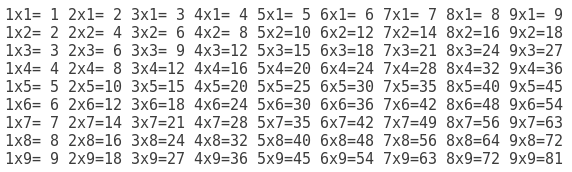
\includegraphics[width=0.9\textwidth]{fig/L5_example_001}
	\label{L5_example_001}
\end{figure}

\subsection{解題思惟}
\begin{enumerate}
	\item 使用兩個for迴圈,第一個用來印出乘號後面的數字,第二個用來印出乘號前面的數字。
	\item 此題需要注意的是,為了使九九乘法表對齊,乘出來的數字要佔兩個位置,因此小於十的乘積需在十位數的地方補一個空格。這個部份使用printf較為簡單,直接使用\%2d的指定格式即可。
\end{enumerate}

\subsection{程式碼}
\begin{cppcode}
	#include <cstdio>
	
	int main()
	{
		for(int i=1; i<10; i++) {
			for(int j=1; j<10; j++) {
				printf("%dx%d=%2d ", j, i, i*j);
			}
			printf("\n");
		}
		return 0;
	}
\end{cppcode}
註:本題在瘋狂程設測試時,限制不能出現\",因此上述程式沒有辦法通過。因為printf第一個參數是字串,會用到\",那我們可以改用cout,然後其他文字都改用字元(字元使用\'而不是\"),這樣的話,程式碼可以改寫如下:
\begin{inside}
	#include <iostream>
	#include <iomanip>
	
	using namespace std;
	
	int main()
	{
		for(int i=1; i<10; i++) {
			for(int j=1; j<10; j++) {
				cout<<j<<'x'<<i<<'='<<setw(2)<<i*j<<' ';
			}
			cout<<endl;
		}
		return 0;
	}
\end{inside}
注意此處輸出乘積的時候,限制輸出寬度為2格,可以引入<iomanip>檔頭,並在cout中使用setw(2)的敘述達成。或者也可以自行判斷,當乘積小於10的時候,先多印一個空白,再輸出乘積。
